\documentclass{article}
\usepackage[utf8]{inputenc}
\usepackage{listings}
\usepackage{graphicx}
\usepackage{xcolor}
\usepackage{amsmath}
\usepackage{bm}
\usepackage[makeroom]{cancel}
\usepackage{float}
\usepackage{hyperref}
\usepackage{caption}
% \usepackage{subfigure}
\usepackage{subfig}
\usepackage[
    style=alphabetic,
    maxbibnames=99,
    maxnames=99
]{biblatex} %Imports biblatex package

\addbibresource{bibliography.bib}

% \lstset{
%     numbersep=5pt,
%     breaklines=true,
%     postbreak=\mbox{\textcolor{red}{$\hookrightarrow$}\space},
%     keywordstyle=\color{red}
% }
\definecolor{codegreen}{rgb}{0,0.6,0}
\definecolor{codegray}{rgb}{0.5,0.5,0.5}
\definecolor{codepurple}{rgb}{0.58,0,0.82}
\definecolor{backcolour}{rgb}{0.95,0.95,0.92}

\lstdefinestyle{mystyle}{
    backgroundcolor=\color{backcolour},   
    commentstyle=\color{codegreen},
    keywordstyle=\color{magenta},
    numberstyle=\tiny\color{codegray},
    stringstyle=\color{codepurple},
    basicstyle=\ttfamily\footnotesize,
    breakatwhitespace=false,         
    breaklines=true,                 
    captionpos=b,                    
    keepspaces=true,                 
    numbers=left,                    
    numbersep=5pt,                  
    showspaces=false,                
    showstringspaces=false,
    showtabs=false,                  
    tabsize=2
}

\lstset{style=mystyle}

\floatplacement{table}{H}
\floatplacement{figure}{H}

\title{Implementation of a library for convolutional neural networks in futhark}
\author{Alexander Nortung}
\date{2022-06-13}

\begin{document}

\maketitle

\section{Neural networks}%
\label{sec:Neural networks}

A neural network is a machine learning model, that consists of a set of layers. Neural networks are used to recognize patterns in data and be able to classify it. The way it works is by having some input data that can be used as a input to the network, and then be propageted through each layer. In an untrained network the output would not make much sense, but by training the network with known input and expected output data, a network can give quite accurate results.

\subsection{Fully connected layer}%
\label{sub:Fully connected layer}

The fully connected layer is also known as a dense layer or a linear layer.
The input can be represented as neurons and synapses, with $D$ input neurons and $M$ output neurons. Each input neuron will be connected by synapses to all output neurons.
This layer's input can be represented as a vector $\bm{x}$ and the output can also be represented as a vector $\bm{y}$.
In \autoref{fig:neural_network} it is illustrated what is the input, a connection and the output.

\begin{figure}
    \centering
    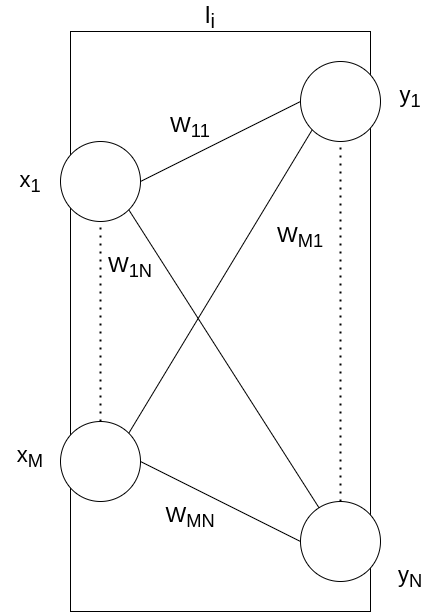
\includegraphics[width=0.5\textwidth]{assets/linear-layer.png}
    \caption{An illustration of a fully connected layer, where the dotted lines means there might be more values in between.}
    \label{fig:neural_network}
\end{figure}


The synapses works by having a weight which is multiplied to the value from the input.
The weights of the synapses can be represented as a matrix $\bm{W}$, which will now be referred to as the weights.
The weight $w_{ij}$ corresponds to the weight between input $i$ and output $j$.
Where $i = 1, ..., D$ and $j = 1, ..., M$.

When data is propagated through this layer, it goes from the input through a synapse, where it is multiplied by the weight and then each value that ends in that output is summed together.

$$y''_j = \sum_{i=0}^D w_{ji}x_i  $$

Once the data has reached the output, there should also be added a bias, which can make the layer be able to fit better to the desired result.
The bias $\bm{b}$ can be represented as a vector with the same length as the output $M$.

$$y'_j = b_j + \sum_{i=0}^D w_{ji}x_i$$

The vector $\bm{y'}$ can thus be represented as a vector to matrix multiplication and adding the bias vector

$$\bm{y'} = \bm{b} + \bm{W}\bm{x}$$

At last there should be applied an activation function, this will be denoted $\sigma$.
So $y_j$ becomes

$$y_j = \sigma \left(y'_j\right)$$

\subsection{Activation functions}%
\label{sub:Activation functions}

Activation functions have an important role in neural networks, since they can introduce non-linearity. This is important when training the network.
Some common activation functions can be seen in \autoref{tab:activation}.

\begin{table}[H]
\centering
\begin{tabular}{|c|c|}\hline
\textbf{Function} & $\bm{\sigma}$ \\\hline
tanh     & $\frac{e^x - e^{-y'}}{e^x + e^{-y'}}$ \\\hline
ReLU     & $max(0, y')$ \\\hline
sigmoid  & $\frac{1}{1+e^{-y'}}$ \\\hline
softmax  & $\frac{e^{y'}}{\sum^K_{k=1} e^{y'_k}}$ \\\hline
\end{tabular}
\caption{A list of common activation functions.}
\label{tab:activation}
\end{table}

\subsection{Convolutional layer}

A neural network with one or more convolutional layers are called a convolutional neural network.
The convolutional layer is often takes a three dimensional input, where the two dimensions can be an image and the third dimension is the channels. The channels of an image is most often the different color channels such as red, green and blue.

The goal of a convolutional layer is to detect certain features, in the given input. The network will be able to detect more and more complex features depending on how many convolutional layers the network has.

The convolutional layer works by having a kernel $\bm{K}$ that convolves through the input. The kernel should not be confused with kernels in cuda, it is also known as a filter. The kernel has the same number of dimensions as the input, but the sizes of the image dimensions of the kernel should be less than or equal to the image dimensions of the input. This can be seen on \autoref{fig:conv_input_and_kernel}.

\begin{figure}
    \centering
    \hfill
    \subfloat[][An example for a $3 \times 3$ input to a convolutional layer]{$\begin{bmatrix}
        X_{11} & X_{12} & X_{13} \\
        X_{21} & X_{22} & X_{23} \\
        X_{31} & X_{32} & X_{33} 
    \end{bmatrix}$}
    \hfill
    \subfloat[][An example for a $2\times 2$ kernel]{$\begin{bmatrix}
        K_{11} & K_{12} \\
        K_{21} & K_{22}
    \end{bmatrix}$}
    \hfill
    \null
    \caption{An example for an input and a kernel to be used in a convolutional layer}
    \label{fig:conv_input_and_kernel}
\end{figure}


The convolutional operation works by taking the dotproduct of the kernel with a slice of the input, then adding a bias and applying the activation function. This is done for each channel with the same slice. These values are then stored in the output. This is repeated for a new slice until the the end of the input. The operaion is visualized in \autoref{fig:conv_operation}, the result will be $\bm{Y}''$, to get $\bm{Y}$ there needs to be added a bias and used an activation function.

\begin{figure}
    \centering
    $$\begin{bmatrix}
        \color{red} X_{11} & \color{red} X_{12} & X_{13} \\
        \color{red} X_{21} & \color{red} X_{22} & X_{23} \\
        X_{31} & X_{32} & X_{33} 
    \end{bmatrix} \otimes K \Rightarrow \begin{bmatrix}
        \color{red} X_{11} K_{11} + X_{12} K_{12} + X_{21} K_{21} + X_{22} K_{22} & \\
         &
    \end{bmatrix}$$\\
    $$\begin{bmatrix}
        X_{11} & \color{red} X_{12} & \color{red} X_{13} \\
        X_{21} & \color{red} X_{22} & \color{red} X_{23} \\
        X_{31} & X_{32} & X_{33} 
    \end{bmatrix} \otimes K \Rightarrow \begin{bmatrix}
         Y''_{11} &\color{red} X_{12} K_{12} + X_{13} K_{13} + X_{22} K_{22} + X_{23} K_{23} \\
         &
    \end{bmatrix}$$\\
    $$\begin{bmatrix}
        X_{11} & X_{12} & X_{13} \\
        \color{red} X_{21} & \color{red} X_{22} & X_{23} \\
        \color{red} X_{31} & \color{red} X_{32} & X_{33}
    \end{bmatrix} \otimes K \Rightarrow \begin{bmatrix}
        Y''_{11} & Y''_{12} \\
        \color{red} X_{21} K_{21} + X_{22} K_{22} + X_{31} K_{31} + X_{32} K_{32} & 
    \end{bmatrix}$$\\
    $$\begin{bmatrix}
        X_{11} & X_{12} & X_{13} \\
        X_{21} & \color{red} X_{22} & \color{red} X_{23} \\
        X_{31} & \color{red} X_{32} & \color{red} X_{33}
    \end{bmatrix} \otimes K \Rightarrow \begin{bmatrix}
         Y''_{11} & Y''_{12} \\
         Y''_{21} & \color{red} X_{22} K_{22} + X_{23} K_{23} + X_{32} K_{32} + X_{33} K_{33}
    \end{bmatrix}$$\\
    \caption{A visualization of the convolutional layer operation. The red numbers on the left are the input values that are currently in the window. The red number on the right is the result of the dotproduct of the window and the kernel.}
    \label{fig:conv_operation}
\end{figure}

To put it as a formula for the 2 dimensional image,
let $\bm{X}$ be the input,
$\bm{Y}$ be the output.
$\bm{b}$ be a vector of the bias with the length equal to the number of output channels.
$C_{in}$ the number of input channels.
$\bm{K}$ the kernel.
$k_x$ and $k_y$ the size of the kernel and $s_x$ and $s_y$ be the stride which the kernel is moving through the image.

$$Y_{ijc_{out_l}} = b_{c_{out_l}} + \sum^{C_{in}}_{c = 1} \sum^{i \cdot s_x + k_x}_{i_2 = i \cdot s_x} \sum^{j \cdot s_y + k_y}_{j_2 = j \cdot s_y} X_{i_2j_2c} K_{i_2j_2c} $$

Where $i$ is the index in the first image dimension, $j$ is the index in the second image dimension and $c_{out_l}$ is the current output chnanel.

$i$, $j$ and $l$ are in the following ranges

$$i = 1, ..., \frac{n_x - k_x}{s_x} + 1$$
$$j = 1, ..., \frac{n_y - k_y}{s_y} + 1$$
$$l = 1, ..., C_{out}$$

Where $n_x$ and $n_y$ are the image dimensions.

This means the dimensions of $\bm{Y}$ is

$$\left(C_{out}\right) \times \left(\frac{n_x - k_x}{s_x} + 1\right) \times \left(\frac{n_y - k_y}{s_y} + 1\right) $$

\subsection{Maxpooling layer}

The max pooling layer splits the input into different windows, and outputs the maximum value in each window. The operation is more easily understood in \autoref{fig:max_pool}.

\begin{figure}[htpb]
    \centering
    $$\begin{bmatrix}
        \color{red}1 & \color{red} 2 & \color{green} 3 & \color{green} 4 \\
        \color{red}8 & \color{red}9 & \color{green}10 & \color{green}11 \\
        \color{blue}7 & \color{blue}1 & \color{magenta}2 & \color{magenta}6 \\
        \color{blue}2 & \color{blue}1 & \color{magenta}9 & \color{magenta}3
        \end{bmatrix} \Rightarrow \begin{bmatrix}
        \color{red}9 & \color{green}11 \\
        \color{blue}7 & \color{magenta}9
        \end{bmatrix}$$
    \caption{Illustration of a max pooling operation on a $4\times 4$ matrix with a $2\times 2$ window. The window will process the numbers of the same color and output the same color.}
    \label{fig:max_pool}
\end{figure}

In this example the first slice will be $[1, 2, 8, 9]$, the slice is flattened for easier readability. Then the greatest number is $9$ which will be set in the output. This is repeated for the next slice and then repeated until the window reaches the end of the input.

The maxpooling layer reduces the input, such that only the most important features are carried over to the next layer and thus reducing the number of operaitons needed for the nect layer.

\subsection{Composition of layers}%
\label{sub:Composition}

A neural network does often not accomplish much with a single layer, that means the network should be a composition of layers. A simple neural network with multiple layers is a multilayer perceptron which is a network with only fully connected layers, this can be seen on \autoref{fig:multilayer_perceptron}.

\begin{figure}
    \centering
    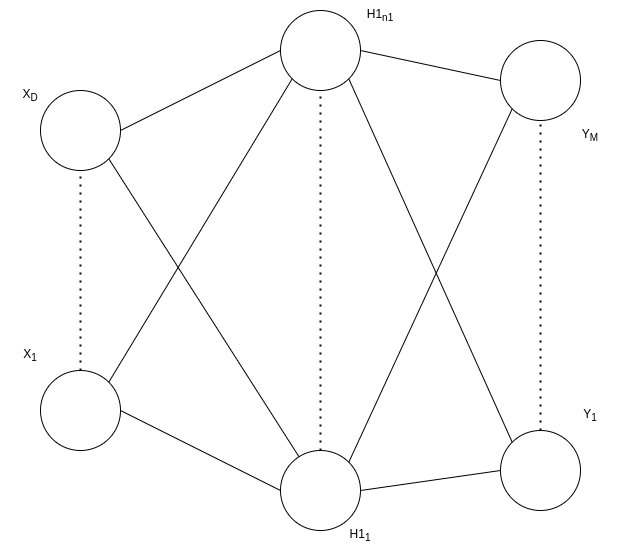
\includegraphics[width=0.6\textwidth]{assets/multilayer-perceptron.png}
    \caption{A multilayer perceptron (a neural network with only fully connected layers). Where $H1_1, ..., H1_{n1}$ are the outputs of the first layer.}
    \label{fig:multilayer_perceptron}
\end{figure}

But the network can be composed how the user likes it, the only restriction is that the number of outputs in one layer has to match with the number of inputs in the next layer. The input for a layer might also need to be transformed from its original shape to the input shape of the next layer.

When composing the layers, the forward propagation function also changes, where the input type will not change, but the output type will be the type of the last layer.
The new forward propagation function will be the following $g_{nnl}$

$$f_{nnl} = f_l(f_{nn})$$

Where $f_l$ is the forward propagation of the layer and $f_{nn}$

\subsection{Loss functions}%
\label{sub:Loss functions}

To determine how close the network is at predicting something, a loss function can be used.
The loss function works by taking the output of the network and comparing it with the expected value or label.
This will be relevant in the following subsection (\autoref{sub:network_training}).

There are different loss functions that finds the loss in different ways. Some common loss functions can be seen in \autoref{tab:loss}

\begin{table}[ht]
\centering
\begin{tabular}{|c|c|}
\hline
\textbf{Loss function}  & \textbf{L(W)} \\ \hline
Cross entropy  & $-\sum^K_{k=1}(l_k\ ln\ y_k)$ \\ \hline
Mean squared error & $\frac{1}{K}\sum^K_{k=1}(y_k-l_k)^2$ \\ \hline
\end{tabular}
\caption{Some common loss functions, where $\bm{y}$ is the output of the network and $\bm{l}$ is the expected values or labels}
\label{tab:loss}
\end{table}

\subsection{Network training}%
\label{sub:network_training}

The goal of using a neural network is to make it correctly classify some input data. This can be done by training the network.
The network can be trained by "optimizing" the weights for each layer. Here optimizing is referred to as giving a better result and not as code optimizing.
One method of optimizing the network is by using gradient descent.
The function $E$ which the gradient will be found, is the forward propagation of the network as a function of the weights, composed with a loss function, which is shown in the following formula.

$$E(\bm{W}) = L(f(\bm{W}_1, \bm{W}_2, ..., \bm{W}_n))$$

Where $n$ is the number of layers in the network, $\bm{W}_i$ is the weights for layer $i$ where $i = 1...n$, $L$ is a loss function and $f$ is the forward propagation.
Gradient descent works because the loss function will be minimized, thus the weights need to change to fit the input and label data.

In \autoref{sec:autodiff} it will be discussed how to find the gradient or derivative of any function, which can be used for gradient descent.

\subsection{Exploding and vanishing gradients problem}

When using the backpropagation algorithm in a neural network, the gradient in some layers might be so small, that when updating the weights of the early layers, they will barely change. This problem is referred to as the vanishing gradients problem, as the gradients become so small that they almost vanish.
This problem makes it much harder to train a network since the weights might never reach the optimal value.
On the other hand the gradients might get so large that they move the weights way too much, such that the weights will never really hit an optimal value.
This problem can make the network significantly harder to train and maybe even impossible. This can, for example, make the application of vanilla SGD impossible \cite{exploding_gradients}.

This problem can be dealt with by using normalization layers which will be discussed in \autoref{sub:norm_layers}.


% There is no well-accepted metric for determining the presence of pathological exploding gradients \cite{exploding_gradients}.

\subsection{Normalizations layers}%
\label{sub:norm_layers}


\subsection{Residual network (ResNet)}

Deep convolutional neural networks have led to a series of breakthroughs for image classification \cite{resnet}.
To solve more and more complex tasks, deeper networks seems to be more accurate.
The problem is that the networks can not just get deeper and deeper since it seems that when a certain limit is reached accuracy is becoming saturated and after adding more layers accuracy seems to degrade.
An obstacle to this problem has also been the problem of vanishing/exploding gradients.
However ResNet is able to be accurate in considerably increased depth and have dealt with the problem of exploding/vanishing gradients by using normalization layers. ResNet also produces results substantially better than previous networks \cite{resnet}.

In this section there will be described which methods ResNet uses and how the model is structured.

% \subsubsection{Residual representation}

\subsubsection{Shortcut connections}

A shortcut connection is a connection that skips one or more layers and may have parameters that change the values.
\autoref{fig:shortcut_connection} shows an example of a shortcut connection that adds the input $\bm{x}$ value of the first layer to the output of the last layer.
Where $F(\bm{x})$ is the forward propagation of the block. The block in this case is just the two weight layers, but in general a block can have any number of layers.
In this case the shortcut connection is an identity mapping, meaning that the connection does not change the value of $\bm{x}$ during the shortcut connection.

\begin{figure}
    \centering
    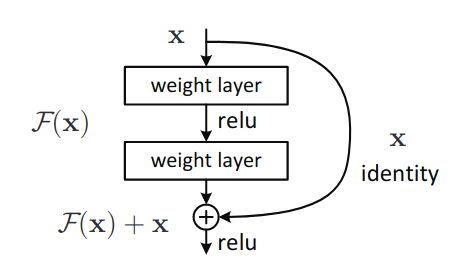
\includegraphics[width=0.55\textwidth]{assets/shortcut-connection.png}
    \caption{A shortcut connection represented by the arching arrow. $\mathcal{F}(\bm{x})$ is the function of applying $\bm{x}$ to the two layers. $\mathcal{F}(\bm{x}) + \bm{x}$ is the value after the shortcut connection. Source: \cite{resnet}}
    \label{fig:shortcut_connection}
\end{figure}

The benefit a shortcut connection is that it deals with the exploding/vanishing gradients problem, since it can allow the gradient to "flow" through to earlier layers, without exploding or vanishing in the same way.

\subsubsection{Deep residual learning}

Residual learning builds on the use of shortcut connections. 
This is done by having shortcuts with identity mapping for every few layers.
The shortcut connections in Eqn.(1) introduce neither extra parameter nor computation complexity \cite{resnet}.
The only extra number of computation that is needed during residual learning is making an element-wise matrix-matrix addition, for every few layers.
The element-wise addition is computationally cheap, thus it can be a very good trade off if it means that the network might be trained faster and it might have better accuracy.

The dimensions of $\bm{x}$ and $\mathcal{F}(\bm{x})$ has to be equal, if they are not the data can be linearly projected by a matrix $\bm{W}_s$ to match the dimensions of $\bm{y} = \mathcal{F}(\bm{x}) + \bm{W}_s\bm{x}$.

\subsubsection{Netwok architecture}%

\textbf{Plain network}: The convolutional layers mostly have $3 \times 3$ filters and follow two simple design rules:
(i) for the same output
feature map size, the layers have the same number of filters; and
(ii) if the feature map size is halved, the number of filters is doubled so as to preserve the time complexity per layer
\cite{resnet}.
Whenever the data nis downsampled it is done by a convolutional layer with a stride of 2.
In the end the network has a fully connected layer with 1000 outputs.

\textbf{Residual network}: 
The residual network is based on the plain network, but uses shortcut connctions

\begin{figure}
    \centering
    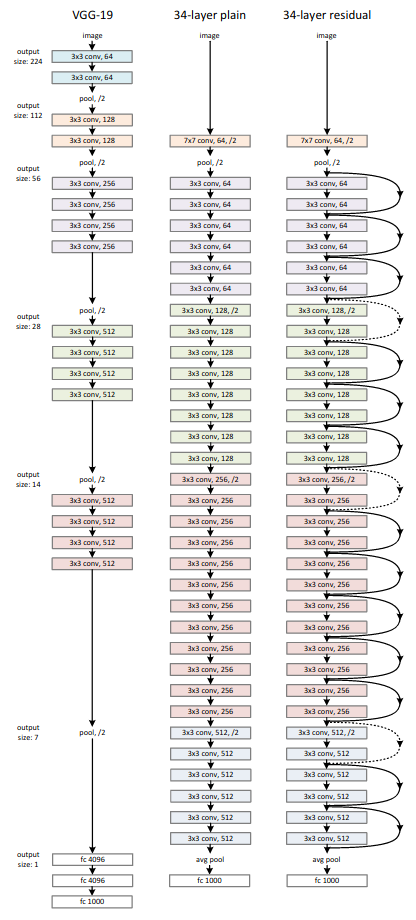
\includegraphics[scale=0.69]{assets/residual-net.png}
    \caption{The first part of each layer tells which type of layer it is, the second tells how many channels the layer uses, and the third tells if there is downsampling ($/2$). \textbf{middle}: 34-layer plain network. \textbf{right}: 34-layer residual network - based on plain, but with shortcut connections. Source: \cite{resnet}}
    \label{fig:resnet}
\end{figure}




\section{Automatic differentiation}%
\label{sec:autodiff}

In \autoref{sub:network_training} it was discussed how a neural network can be trained to classify sets of data. To train the network one would need to find the derivative of the loss function. A simple way this can be done is by manually finding the derivative of each function and use those
% TODO: vær sikker på at dette er korrekt
and applying the chain rule.

However when looking at this from a software engineering perspective it might be much more work to find the derivative of each function and if anything is changed in any of the functions, the derivative would also have to be changed, thus requiring more maintainance.

A solution to this is automatic differentiation, which is a method used by the Futhark compiler to make transformations to functions into their derivative.

\subsection{Methods of differentiation}

Before going into detail on how automatic differentiation it is good to know what other methods could be used and what the advantages and disadvantages are.

First there is manual differentiation, where the derivative is found by hand.

Second there is numerical differentiation, where the derived value is approximated by using the original function. This is done by taking the point $\bm{x}$ and the point $\bm{x}+h$ where $h>0$ is a very small real number. To approximate a gradient $\nabla f = \left(\frac{\partial f}{\partial x_1}, ..., \frac{\partial f}{\partial x_n} \right)$ the following formula can be used
$$\frac{\partial f(\bm{x})}{\partial x_i} \approx \frac{f(\bm{x} + h\bm{e}_i) - f(\bm{x})}{h}$$
Where $\bm{e}_i$ is the $i$-th unit vector. This can be very easy to implement, however to find the derivative for $n$ dimensions the performance would be $O(n)$ \cite{autodiff}.

Third there is symbolic differentiation, this is what many math programs such as maple use. It is an automatic manipulation of an expression that obtains a derivative expression. The derivative expression is obtained by systematically applying rules.
A problem with symbolic differentiation is that the symbolic structure is not necessarily efficient in runtime computation since symbolic derivatives can get exponentially larger
\cite{autodiff}.

\subsection{Automatic differentiation}%
\label{sub:autodiff}

Automatic differentiation can be used when we do not need the derivative's symbolic form.
A function's symbolic form can for example be $f(x) = sin(x) * 2$.
In automatic differentiation it is not needed to be this verbose, this is because the code will eventually just return a numeric value anyway.
Since we do not need the derivative's symbolic form it is possible to significantly simplify the computations and by storing only the values of intermediate sub-expressions in memory \cite{autodiff}. Another advantage of using automatic differentiation over the other ones is that we can use branching and loops.

\subsubsection{Forward mode}

Automatic differentiation in forward mode is conceptually the most simple type \cite{autodiff}. In forward mode the derivative is found whenever a variable is defined, consider a function
$y = f(g(h(x)))$, and as variables
\begin{lstlisting}
w0 = x
w1 = h(w0)
w2 = g(w1)
w3 = h(w2)
y = w3
\end{lstlisting}
now the derivative will can be found by computing the derivative of each variable in the order it was declared.
$$y' = \frac{\partial y}{\partial x} = \frac{\partial y}{\partial w_2} \frac{\partial w_2}{\partial x} = \frac{\partial y}{\partial w_2} \left(\frac{\partial w_2}{\partial w_1} \frac{\partial w_1}{\partial x}\right) = \frac{\partial y}{\partial w_2} \left(\frac{\partial w_2}{\partial w_1} \left(\frac{\partial w_1}{\partial w_0} \frac{\partial w_0}{\partial x}\right) \right)$$
Since $w_0 = x$ and $\frac{\partial x}{\partial x}$, it does not make sense to go any further and the expression can be reduced to
$$y' = \frac{\partial y}{\partial w_2} \left(\frac{\partial w_2}{\partial w_1} \left(\frac{\partial w_1}{\partial x}\right) \right)$$.

As an example consider this function $r = F(x, y) = \sin(x) + x\cdot y$, Where the derivative is found with respect to $x$.
\begin{lstlisting}[label={lst:autodiff_fwd_trace}, caption={Forward trace of a simple function $f(x, y) = \sin(x) + x\cdot y$}]
w0 = x
w1 = sin(w0)
w2 = w0 * y
w3 = w1 + w2
r = w3
\end{lstlisting}
$$r' = \frac{\partial r}{\partial w_2} \left(\frac{\partial w_2}{\partial w_1} \left(\frac{\partial w_1}{\partial x}\right) \right)$$.
Now each intermediate derivative can be solved.
\begin{lstlisting}[label={lst:autodiff_fwd_deriv}, caption={Forward derivative trace of a simple function $f(x, y) = \sin(x) + x\cdot y$}]
w0' = 1
w1' = cos(w0) * w0'
w2' = y
w3' = w1' + w2'
r' = w3'
\end{lstlisting}
To verify $r'$ can be show to reduce to $r' = \cos(x) + y$.

Automatic differentiation in forward mode differentiates each expression as it reaches them in \autoref{lst:autodiff_fwd_trace} which can be seen in \autoref{lst:autodiff_fwd_deriv}. This is done for each input parameter, so in the previous example $\frac{\partial r}{\partial x}$ and $\frac{\partial r}{\partial y}$ is found.

For $n$ input parameters and a function $$F(x_1, ..., x_n) = [ y_1, ..., y_m ]$$ that returns $m$ outputs, the Jacobian can be calculated. For each input parameter and each output value the derivative needs to be found in order to find the Jacobian.
$$\bm{J}_F = \left[
  \begin{array}{ccc}
    \frac{\partial y_1}{\partial x_1} & \cdots & \frac{\partial y_1}{\partial x_n}\\
    \vdots & \ddots & \vdots\\
    \frac{\partial y_m}{\partial x_1} & \cdots & \frac{\partial y_m}{\partial x_n}\\
  \end{array}
\right]$$
This Jacobian can be computed in $n$ iterations, one iteration for each forward trace or input parameter.
The derivative values at point $\bm{r}$ by simply multiplying $\bm{r}$ to the Jacobian $\bm{J}_F$.

\subsubsection{Reverse mode}%
\label{ssub:reverse_mode}








\section{Design and implementation}

The implementation was created using Futhark, Futhark is a functional language which focuses on compiling effecient parallel code.
Futhark comes with some limitations, one being that arrays cannot be irregular or contain functions.
If this limitation was not there, it would be easy to make an array of the functions for each layer and then use a \texttt{fold}-like operation for the forward propagation.

\subsection{Design}

The design idea was to implement each layer as a module that could calculate the forward propagation and update the weights given a gradient.
The idea of combining layers into a network was part of the design early on.
This meant that there needed to be a way to store the forward propagation function and the weights of the entire network.
It was also important that the weights could be given as a single argument to the network, since that would be used for the automatic differentiation function \texttt{vjp}. The type of \texttt{vjp} can be seen in the following listing.
\begin{lstlisting}
val vjp 'a 'b : (f: a -> b) -> (x: a) -> (y': b) -> a
\end{lstlisting}

This then lead to the idea of storing the forward function and weights in a record like the following. It should also be important to store a function that can apply the gradient to the weights, in this project it is called \texttt{apply\_optimize}.

\begin{lstlisting}
type^ nn_type 'input 'output 'current_weight 'rest_weights = {
  forward: input -> (current_weight, rest_weights) -> output,
  apply_optimize: (current_weight, rest_weights) -> (current_weight, rest_weights) -> (current_weight, rest_weights),
  weights: (current_weight, rest_weights)
}
\end{lstlisting}

This means that it is easy to add a new layer to the network by simply composing the \texttt{forward} function, \texttt{apply\_optimize} function and adding the weights of the current layer to the \texttt{current\_weight} part of the \texttt{weights} tuple.
It also means it is easy to call the forward propagation of the network with some input.

In \autoref{lst:add_layer} it can be seen how layers can be composed in a simplified way.

\begin{lstlisting}[caption=A simplified version of adding a layer to a network, label={lst:add_layer}]
def add_layer (layer) (network) =
  let {
    apply_optimize = layer_apply_optimize,
    forward = layer_forward,
    weights = layer_weights,
  } = layer
  let { apply_optimize, weights, forward } = network
  let new_forward = (\input (cw, rw) -> layer_forward (forward input rw) cw)
  let new_apply_optimize = (\(cw, rw) (cg, rg) -> (layer_apply_optimize cw cg, apply_optimize rw rg)
  in {
    weights = (layer_weights, weights),
    apply_optimize = new_apply_optimize,
    forward = new_forward
  }
\end{lstlisting}

To add layers to a network, the network needs to be initialized, the way the network is initialized is by setting the \texttt{forward} and \texttt{apply\_optimize} functions as an identity functions of the input and keep the weights as two empty tuples \texttt{((), ())))}.

It is also important that layers follow the same type, so they work with the \texttt{add\_layer} function, the type of layers can be seen in the following listing.

\begin{lstlisting}
type^ layer_fwd_type 'options 'layer_input 'wb 'out = options -> layer_input -> wb -> out
type^ layer_apply_optimize_type 't 'apply 'options 'weights = options -> apply -> weights -> weights -> weights
type^ layer_type 't 'options 'layer_input 'wb 'shape 'out = {
  forward: layer_fwd_type options layer_input wb out,
  apply_optimize: layer_apply_optimize_type t options wb,
  options: options,
  weights: wb,
}
\end{lstlisting}

Here \texttt{layer\_fwd\_type} is the type of the forward function inside a layer. In \texttt{layer\_type} there is also a field for \texttt{options}, this can be different for different layer type, but can as an example contain information about strides or padding.

\subsection{Interface}

One part of the design was to make the interface as easy to use as possible, this was attempted by adding a \texttt{shape} field for the neural network type. The intention with this field was that it could be used to define the input shape of the next layer, in such a way that the user could avoid having to manually type in the output sizes of some layers. However due to limitations of Futhark it was not possible to use a field in a record to define size types. The intended way to this would be something like the following listing.

\begin{lstlisting}[caption=the \texttt{add\_layer} function but with an added field \texttt{shape}.]
def add_layer (layer) (network) =
  let {
    apply_optimize = layer_apply_optimize,
    forward = layer_forward,
    weights = layer_weights,
    shape = layer_shape,
  } = layer
  let { apply_optimize, weights, forward, shape } = network
  let new_forward = (\input (cw, rw) -> layer_forward (forward input rw) cw)
  let new_apply_optimize = (\(cw, rw) (cg, rg) -> (layer_apply_optimize cw cg, apply_optimize rw rg)
  in {
    weights = (layer_weights, weights),
    apply_optimize = new_apply_optimize,
    forward = new_forward,
    shape = layer_shape
  }
\end{lstlisting}

Here the \texttt{shape} field could define the output shape of the network and we could destructure the layer in the parameters and use the shape values in the return type.

The interface for the layers will be described more in \autoref{sub:layers}

\subsection{Library structure}

In this section an overview of the library structure will be given.

The largest part of the library is contained within one module with multiple submobules, the reason for this is that it provides a nice interface and the user of the library would not have to import each feature that they need.
The idea is that the user can import \texttt{neural-network/neural-network} as a module that can be called \texttt{nn}, and then access close to the entire library.

Layers are each defined in their own module, this makes sense since there are much functionality and many components that should only be used in one place, so naturally it makes sense to separate it it.
Layers can be accessed by the user in \texttt{nn.layers} and are defined in the \texttt{layers/} directory.

\subsection{Activation functions}

Activation functions in this implementation is simple and its type is represented as the following

\begin{lstlisting}[caption=The type definition of activation functions., label={lst:activation_type}]
type^ activation_type 't = (n: i64) -> [n]t -> [n]t
\end{lstlisting}

The reason that \texttt{n} needs to be given as an argument is that otherwise Futhark might try to generalize \texttt{n}, which would result in compilation errors when having multiple layers of different output sizes.

The activation functions can be accessed by the user in \texttt{nn.activation}.

The user can also define their own activation functions and use them as long as they follow the type described in \autoref{lst:activation_type}.

\subsection{Loss functions}

The loss functions are used in a different way than activation functions. A loss function of the network can be defined be using the function \texttt{nn.make\_loss}, this function should return a function that takes an array of inputs and an array of labels and return an array of errors. The loss functions type is defined as the following

\begin{lstlisting}
type^ loss_type 'input 'labels 't = [k]input -> [k]labels -> [k]t
\end{lstlisting}

The user can also define their own loss functions if the library does not provide it. The user defined loss function can also be given to the \texttt{nn.make\_loss} function.

\subsection{Optimizers}

Optimizers are the modules that perform the backpropagation of the network.
This has been separated as its own module type to allow for new or future implementations of optimizers.

The idea with optimizers is to hold the loss function together with a function that can apply the gradient to the weights of each layer.
Then the optimizer can be given to the \texttt{nn.train} function which performs the actual training. When each layer needs to be updated they will be given an \texttt{apply\_gradient} function, which each layer can call and get an updated weight.
In the current implementation, instead of having a single \texttt{apply\_optmize} function it has a record of 4 different functions, which works on arrays of different dimensions. However this should probably only have been a single function that would take a one-dimensional array, since that would make it easier to maintain and create new optimizers and it is unnecessary complex.

One of the obstacles that was encountered when implementing the \\% Force newline
\texttt{apply\_gradient} function is that the compiler tried to generalize the size types. Consider the following type
\begin{lstlisting}
type^ optimizer_apply_optimize_func 'wb = wb -> wb -> wb
\end{lstlisting}
This function is then passed to the entire network's \texttt{apply\_optimize} function, and for each layer the same function is used.
The problem arises when the Futhark compiler tries to figure out what the type of the function is.
For example, for one layer \texttt{'wb} might have the type \texttt{[5][5]f64} and for another layer \texttt{[8][5]f64}.
In this example the types differ and the Futhark compiler cannot generalize the type of the function.
The solution was to make the type depend on an input parameter, which can be seen in the following listing
\begin{lstlisting}
type apply_1d 't = (a: i64) -> optimizer_apply_optimize_func ([a]t)
\end{lstlisting}

There is implemented one optimizer, which performs gradient descent this module is called \texttt{sgd} and can be accessed in \texttt{nn.optim.sgd}.

\subsection{Layers}%
\label{sub:layers}
% Layers
% Unit tests
% Interface

There are implemeted three types of layers, the fully connected layer (\autoref{ssub:impl_fully_connected}), max pooling (\autoref{ssub:impl_max_pool}) and convolutional (\autoref{ssub:impl_conv}).
To make sure the implementation works with different layers that out put different shapes and dimensions, there is also implemented a layer that transforms the output of the previous layer to the shape the user likes. This layer will be described in \autoref{ssub:impl_dimension}.

In the implementation a few shorthand functions have been added to easily add basic layers to the network, these will be described in the following subsubsections.

\subsubsection{Fully connected}%
\label{ssub:impl_fully_connected}

The fully connected layer is initialized with the function \texttt{nn.layers.linear.init} which is a function that takes \texttt{m} and \texttt{n} as its input and output size, an activation function and a seed for initializing weights.
The bias and weights can be set by the user by using the functions \texttt{nn.layers.linear.set\_bias} and \texttt{nn.layers.linear.set\_weights}, this might be useful if the user already trained a network and wants to set teh weights and bias to use the trained network without training it again.

A shorthand function for adding a linear layer ot a network is by using the functions \texttt{nn.linear}, this function takes a parameter \texttt{n} which is the output size, an activation function and the network the linear layer should be added to. This function is handy since it is very easy to compose multiple layers, with very little code. Here is an example

\begin{lstlisting}
nn.init_1d 5 1
|> nn.linear 8 (nn.activation.relu)
|> nn.linear 6 (nn.activation.relu)
\end{lstlisting}

This makes sure that the user does not need to manually input the input sizes for each layer which could lead to errors if the user is not careful.
To illustrate the difference it makes the following example shows the exact same network, but by using the \texttt{add\_layer} function and initializing each layer manually.

\begin{lstlisting}
let net = nn.init_1d 5 1
let net = nn.add_layer (nn.layers.linear.init 5 8 (nn.activation.relu) net.seed) net
|> nn.add_layer (nn.layers.linear.init 8 6 (nn.activation.relu) net.seed)
\end{lstlisting}

However in the first example, the user will not be able to set the weights and bias, but they will in the second example.

In terms of performance the operation is basically just a matrix-vector multiplication, recall the formula from \autoref{sub:Fully connected layer}
$$\bm{y} = \bm{\sigma} \left( \bm{b} + \bm{W} \bm{x} \right)$$
But since the implementation works on batches or multiple inputs, this can pratically be turned into a matrix-matrix multiplication
$$\bm{Y} = \bm{\sigma} \left( \bm{B} + \bm{W} \bm{X} \right)$$
Where $\bm{Y}$ is a matrix of outputs built from the outputs $\bm{y}$ and $\bm{X}$ is a matrix of inputs built from the outputs $\bm{x}$. $\bm{B}$ would then be the bias vector $\bm{b}$ copied $k$ times to match the size $\bm{Y}$.
Now $\bm{\sigma}$ should only be applied on each column vector in the matrix instead of the entire matrix.
This could give better performance since there are ways to optimize matrix-matrix multiplication a lot.
In an implementation of this, $\bm{b}$ could probably just be added to $\bm{WX}$ by using a \texttt{map}-like function.
However in the current state of the implementation this is not implemented, but should be very easy to implement.

\subsubsection{Max pooling}
\label{ssub:impl_max_pool}

The max pooling layer is straight forward to implement, for each slice of the input the maximum element should be found.
In regard to the interface, the intention was to let the user define the window width and height.
However due to Futhark's limitation on return sizes it made more sense to let the user give the output sizes instead.
This layer can be instantiated with different dimensions with \texttt{init\_1d} and \texttt{init\_2d}.

The \texttt{init\_2d} function takes \texttt{output\_m} and \texttt{output\_n}, which is the size of the output.
The window sizes is then calculated by an integer division which can be seen in the following listing.
\begin{lstlisting}
let window_width = m / output_m
let window_height = n / output_n
\end{lstlisting}
Where \texttt{m} and \texttt{n} are the input sizes.

\subsubsection{Convolutional}
\label{ssub:impl_conv}

The current implementation of the convolutional layer is very simple. \autoref{lst:conv_forward} shows a simplified way of how the convolutional layer works for a two-dimensional input.

\begin{lstlisting}[label={lst:conv_forward}, caption=A simplified forward function for the 2d convolutional layer. Where \texttt{a} and \texttt{b} are the sizes of the kernel.]
let c = a * b
map (\batch ->
  map2 (\filter_out_channel bias_channel ->
    map (\x ->
      map (\y ->
        map2 (\in_channel filter_in_channel -> -- the current in channel
          let input_slice = in_channel[x:x+a,y:y+b]
          let flat_slice = flatten_to c input_slice
          let flat_filter = flatten_to c filter_in_channel
          in lalg.dotprod flat_slice flat_filter
        ) batch filter_out_channel
        |> R.(sum)
        |> (+bias_channel)
      ) ys
    ) xs
  ) filter_weights bias
  |> flatten_3d batch
  |> activation_func (out_channels * output_m * output_n)
  |> unflatten_3d out_channels output_m output_n
) input
\end{lstlisting}

The \texttt{filter\_weights} is an array of the kernels where each kernel is three dimensional (\texttt{out\_channels}, x, y).
\texttt{xs} and \texttt{ys} are arrays that are generated by \texttt{iota}, an example can be seen in the following listing

\begin{lstlisting}
let xs = iota output_m -- m - a + 1
\end{lstlisting}

Since Futhark cannot return size types based on arithmetic for example $m - a + 1$, that means the user has to provide the output size, in this example \texttt{output\_m}.

The convolutional layer can be instantiated with multiple functions, there is \texttt{init\_1d} and \texttt{init\_2d}, each depending on the shape of the input.
\texttt{init\_1d} instantiates a layer that takes a two-dimensional array as input, where the first dimension is the channels.
\texttt{init\_1d} is instantiated with the follwing parameters
\begin{itemize}
    \item \texttt{output\_n}: the output size of the input.
    \item \texttt{in\_channels}: the number of input channels of the input.
    \item \texttt{out\_channels}: the number of channels the output should have, this also means how many kernels the layer should have.
    \item \texttt{kernel\_sz}: The size of the one-dimensional kernel.
    \item \texttt{activation\_func}: The activation function for the layer.
    \item \texttt{seed}: The seed to use for initializing weights.
\end{itemize}
For \texttt{init\_2d} it is the same as \texttt{init\_1d}, but instead of \texttt{output\_n} there is \texttt{output\_m} and \texttt{output\_n}. And instead of \texttt{kernel\_sz} there is \texttt{kernel\_x} and \texttt{kernel\_y}.

This layer type also have shorthand functions, for example \texttt{nn.conv\_2d} which takes the same parameters as \texttt{init\_2d}, but not \texttt{in\_channels}, or \texttt{seed} since they are implicit from the network.

\subsubsection*{Optimizing convolutional layers}

It is possible to optimize the convolutional operation, this can be done in different ways where each has its own strength and weaknesses.
This implementation does not include these optimizations, but could be implemented in future work.

\cite{perfomance_analysis_cnn} describes different convolution algorithms.
The method used in this project is direct convolution, which is slow compared to the other algorithms.

A simple way to optimize the convolution operation is by changing the operation into a matrix multiplication. \autoref{fig:conv_matrix} shows how this can be done by transforming the input data into matrices, where each original slice is converted into a row and the kernels are transformed into columns. Then the two matrices can be multiplied and then transformed into feature maps. This approach is called Generic Matrix-Matrix multiplication (GEMM). The only tradeoff is that this approach has to use more auxiliary memory than the direct convolution.
The performance gain comes from the matrix multiplication which can be performed much faster on a GPU since it can utilize local memory which has low latency and high bandwidth. Optimization of matrix multiplication is described more in \autoref{sec:matmul}.

\begin{figure}
    \centering
    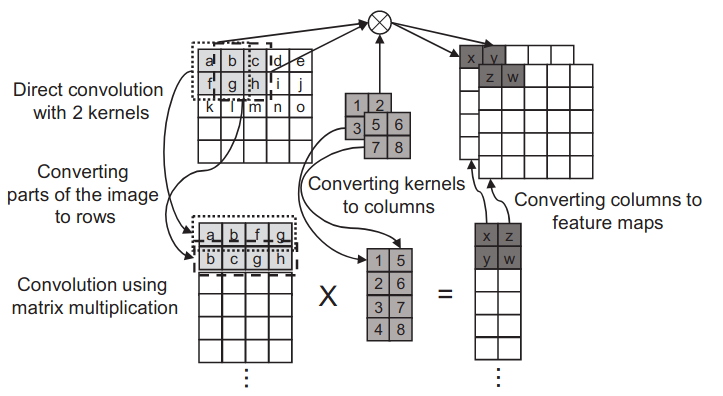
\includegraphics[width=0.9\textwidth]{assets/conv-matrix.png}
    \caption{Direct convolution is shown in the top. The transformed data and kernel for using matrix multiplication is shown in the bottom, and the arrows shows how they aretransformed. Source: \cite{perfomance_analysis_cnn}}
    \label{fig:conv_matrix}
\end{figure}

One way to optimize convolution is by using fast Fourier transform (FFT). The FFT convolution can be used to reduce the computational complexity to $O(K\times CWW \times \log W)$, which does not depend on the kernel size, however it only works with a stride of one \cite{perfomance_analysis_cnn}.
Another way to optimize the convolution operation is by using the Winograd algorithm. The Winograd algorithm is based on GEMM, it reduces multiplication operations significantly when the kernel size is fixed \cite{perfomance_analysis_cnn}. The algorithm gains performance by pre-computing matrices before using matrix multiplication. Since it needs to pre-calculate matrices it works best for small kernel sizes.

% It has been known since at least 1980 that the minimal
% filtering algorithm for computing m outputs with an $r$-tap
% FIR filter [...] requires
% $$\mu (F(m,r)) = m + r - 1$$
% multiplications \cite{fast_conv}.


\subsubsection{Dimension}%
\label{ssub:impl_dimension}

The dimension layer is a helper layer which for example makes it possible to transform the input data from one-dimensional to two-dimensional.
It works for inputs with dimensions between 1d and 3d. The layers have the following naming format \texttt{from\_\textit{x}d\_\textit{y}d} where \texttt{x} can be replaced with the input dimension and \texttt{y} can be replaced with the output dimension. For example \texttt{from\_3d\_1d}.

In the current implementation, a lot of nested \texttt{map}ping is used, however it could probably have been made more effecient by using the builtin \texttt{flatten} function.

The dimension layers are in the module \texttt{nn.dimension}.



\printbibliography

\end{document}
